\section{Disparity Estimation and Scene Flow}
Disparity is the signed distance between images of the same 3D point in two views. Thus it is a special case of optical flow.\\

\b{Comparison to optical flow:}
\begin{itemize}
    \item Disparity is a scalar function rather than a vector field due to the epipolar constraint (1D-Problem)
    \item Makes optimization much easier
    \item Usually we want much larger displacements (more accurate depth)
    \begin{itemize}
        \item Local optimization becomes problematic
        \item Occlusion is more relevant
    \end{itemize}
    \item Disparity estimation has been dominated by combinatorial techniques, now by deep networks
\end{itemize}

\b{Goal/Idea:} Search in both pictures for corresponding points to calculate the difference. It would be easier to find the pixel in second image if we only had to search in one row \f{\to} Transformation of image(s) to have parallel epipolar lines.\\

\b{Special stereo setting:} Using a stereo camera, the camera motion is (approx.) a translation parallel to the x-Axis. Thus the epipolar lines are the image rows.

\subsection{Rectification}
\b{Goal:} Turn a general camera setting into special case with epipolar lines being horizontal scan lines. Can be done by mapping the individual image planes to a plane parallel to the baseline: \f{x'=Hx} (described by homography). Note that the homography shifts the epipoles to infinity. In case the epipole is visible in the image, a polar representation is needed (changes size/dimensions of points but makes epipolar lines parallel).\\

\b{Estimation of rectifying homography:\\[0.5em]}
Given the F-matrix \f{F} we want to find out the rectifying homography \f{H}:
\begin{enumerate}
    \item Get the epipole \f{e'} from \f{F} by solving \f{e'^\top F=0}.
    \item Find out transformation that maps epipole to \f{e'=(1,0,0)^\top}: \f{He'=(1,0,0)^\top}
    \begin{itemize}
        \item Leaves 5 degrees of freedom
        \item Additional constraint: minimize distortion around a point of interest \f{x_0}
    \end{itemize}
    \item Optional: Take both image planes into account, choose a new plane to map to, calculate and minimize the average distortion of both images (requires point correspondences6)
\end{enumerate}

\subsection{Overview of Methods}
\b{Variational methods:}
\begin{itemize}
    \item Removing the v-component from optical flow methods (rectified)
    \item Optimization for non-rectified images possible
    \item Local optimization suboptimal due to large displacements
\end{itemize}
\newpage
\b{Combinatorial optimization:}
\begin{itemize}
    \item Line-wise message passing (rectified)
    \item Semi-global matching
\end{itemize}
\b{Deep Learning:} DispNet (special case of FlowNet)

\subsection{Variational Methods for non-rectified Images}
As the images are not rectified, we need to include the epipolar constraint in the optical flow method.\\
The epipolar line is usually defined as:
\cf{
    l'(x) = Fx =: \begin{pmatrix}
        a(x)\\b(x)\\c(x)
    \end{pmatrix}
}
Then the optical flow vector \f{w:=(u,v)^\top} can be expressed through the disparity \f{d(x)} along the epipolar line \f{l'(x)}. With this the optical flow energy functional can be modified to:
\cf{
    E(d)=\int_\Omega\Psi\left((I_2(x+w(d)))-I_1(x)^2\right)+\alpha\Psi\left(|\nabla d|^2\right)dx
}
\b{Advantage:} Subpixel accuracy. However, results are not convincing.

\subsection{Similarity Measures}
The requirements are similar to optical flow estimation, such as:
\begin{itemize}
    \item Robustness to illumination changes is important
    \item Matching only small patches (ideally pixels) or learned features to ensure high accuracy
\end{itemize}

However, there are some differences too:
\begin{itemize}
    \item Appearance changes are only due to viewpoint, no temporal effects
    \item Global illumination changes are rare
    \item Mostly local reflectance changes due to non-Lambertian surfaces
    \item Occlusion areas tend to be much larger
    \item Occlusion can be derived from the disparity estimate
\end{itemize}

The sum of squared differences compares the color of two batches in the left and right image and is thus sensitive to different reflectance. \f{\to} Use gradient instead of color.\\

\b{Normalized cross correlation} is a similarity measure that is invariant to additive and multiplicative intensity changes. The results are in the range \f{[-1;1]}, where -1 stands for anti-correlation and 1 stands for correlation. To avoid problems in areas without structure, a small constant is added to the denominator. This leads to homogeneous patches having 0 correlation.

\subsection{Combinatorial Optimization}
Combinatorial optimization has been the standard for disparity estimation before being replaced by DL.\\

\b{Message Passing\\[.5em]}
In general the energy on a graph with nodes \f{p}, neigboring nodes \f{q}, pixel labels \f{x\in\{1,...,L\}} and cost \f{\theta} is given by:
\cf{
    E(x) = \sum_p\theta(x_p)+\sum_{p,q\in\mathcal{N}(p)}\theta_{pq}(x_p,x_q)
}
For disparity estimation the labels \f{x} correspond to the disparities, the unary cost \f{\theta(x_p)} is the matching cost and the pairwise cost \f{\theta_{pq}} is a smoothness constraint (neigbors should have similar disparities).\\
If the graph is a tree, a global optimimum can be found by message passing via a forward and backward sweep.\\

The problem can be simplified by estimating the disparity in each image row independently:
\begin{itemize}
    \item Smoothness only in x-direction
    \item Graph in each row is a chain (tree) \f{\to} message passing applicable
    \item Drawback: No smoothness in y-direction
\end{itemize}
\vspace{0.5em}
\b{Semi-Global Matching (SGM)\\[.5em]}
SGM extends the previous approach by considering lines in multiple directions, where each line is still a message passing problem on a chain. For each pixel, the messages from all directions have to be considered.\\

\b{Note:} This is not globally optimal (loops are ignored), but a good approximation.\\

SGM consists of two parts:
\begin{itemize}
    \item Matching costs
    \item Optimization along scan lines
\end{itemize}

\subsection{Deep Networks for Disparity}
\b{SGM with Cost from Deep Network\\[.5em]}
The matching cost for the SGM method can be computed with a siamese network (two heads), which was trained on matching and non-matching patches. Thee network then learns the feature representations of the patches and the metric to compare them.\\

\b{Advantage:} Removes the need for choosing a (suboptimal) metric.\\
\b{Drawback:} One full network pass is needed for each patch comparison.\\

\b{Disparity Networks:\\[.5em]}
Very similar to the original FlowNet structure, can compute the full disparity map at once. The correlation layer inside the network yield a cost volume. The rest of the network then interprets the result of the cost volume.
\newpage
Advantages:
\begin{itemize}
    \item Interactive frame rates on the GPU
    \item Exploits global context between the images (no patch sizes involved)
    \item Outputs are real numbers: no accuracy limit due to quantization
    \item The networks learns how to deal with ambiguities
\end{itemize}

\subsection{Scene Flow}
Scene flow (for videos!) includes depth estimation, optical flow estimation, and estimation of the change in depth. \f{\to} Yields 3D point and its 3D motion vector.\\

Scene flow can be optimized just as optical flow, but this comes with the downside of being supoptimal for stereo. 
Instead, we can separate the depth estimation by applying SGM, which is also applicable directly to RGB-D videos.\\

Deep Networks for scene flow are a combination of FlowNets and DispNets.
\vspace{2cm}
\begin{figure}[h!]
    \centering
    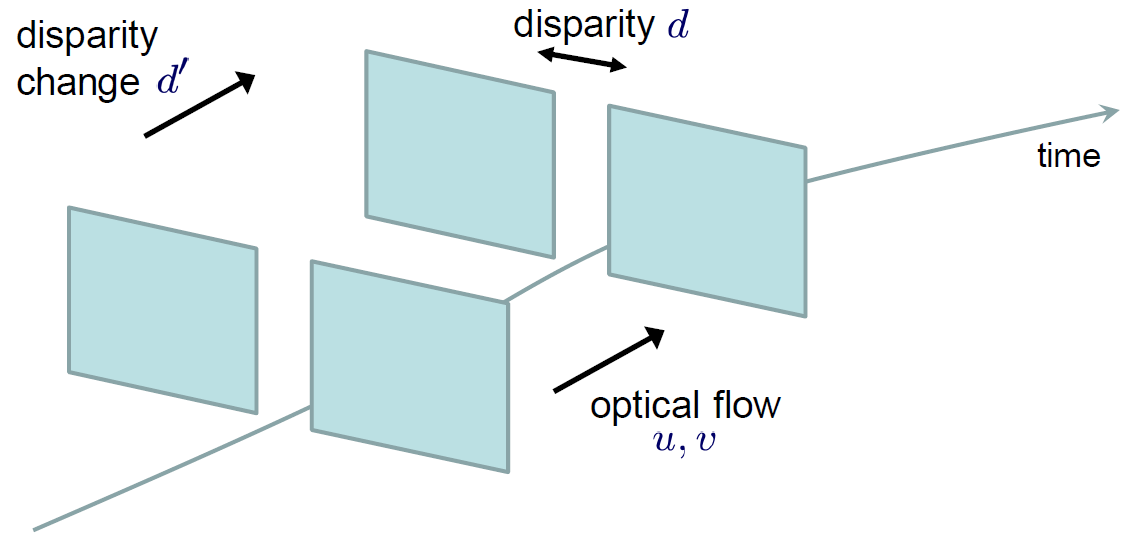
\includegraphics[width=.6\textwidth]{scene.png}
\end{figure}

\newpage